\documentclass[12pt,oneside]{fithesis2}
\usepackage[english]{babel}
\usepackage[latin2]{inputenc}
\usepackage{cmap}
\usepackage[T1]{fontenc}
\usepackage{makeidx}
\usepackage[pdftex]{graphicx}
\usepackage{lmodern}
\usepackage{csquotes}
\usepackage{tabularx}
%\usepackage[bottom]{footmisc}
% \usepackage[round,authoryear,longnamesfirst]{natbib}
\usepackage{url}
\usepackage{caption}
\usepackage{listings}
\usepackage{color}
\usepackage[pdftex,bookmarks=true]{hyperref}
\usepackage{microtype}

\clubpenalty=300
\widowpenalty=300


% english university/faculty name
\renewcommand{\facultyname}{Faculty of Informatics}
\renewcommand{\universityname}{Masaryk University}

\graphicspath{ {./resources/} }

% hyperref
\hypersetup{
    pdftitle={Modern Performance Tools Applied},
    pdfauthor={Ron �meral},
    pdfkeywords={performance testing, performance evaluation, stress testing, load testing, workload modelling},
    linktocpage=true
}

% inline listings
\newcommand{\inlinelisting}{%
\lstset{%
    basicstyle=\ttfamily\small,%
    frame=b,%
    xleftmargin=17pt,%
    framexleftmargin=17pt,%
    framexrightmargin=5pt,%
    framexbottommargin=4pt,%
    aboveskip=\bigskipamount,%
    belowskip=\bigskipamount,%
    keywordstyle=\color{blue},%
    commentstyle=\color{black},%
    columns=fullflexible}}

\lstloadlanguages{
	bash,
    Java, 
    XML
}

% XML listing
\newcommand{\xmllisting}{%
\lstset{%
    basicstyle=\ttfamily\footnotesize,%
    xleftmargin=0pt,%
    framexleftmargin=0pt,%
    framexrightmargin=0pt,%
    framexbottommargin=0pt,%
    keywordstyle=\color{blue},%
    commentstyle=\color{black},%
    columns=fullflexible,%
    showstringspaces=false,%
    commentstyle=\color{gray}\upshape,%
    frame=n,%
    breaklines=true}}

% listings language
\definecolor{gray}{rgb}{0.4,0.4,0.4}
\definecolor{darkblue}{rgb}{0.0,0.0,0.6}
\definecolor{cyan}{rgb}{0.0,0.6,0.6}
\lstdefinelanguage{XML}{
    morestring=[b]",
    morestring=[s]{>}{<},
    morecomment=[s]{<?}{?>},
    stringstyle=\color{black},
    identifierstyle=\color{darkblue},
    keywordstyle=\color{cyan},
    morekeywords={ThreadGroup, stringProp, elementProp, boolProp, intProp}
}

% captions for listings
\DeclareCaptionFont{listing-caption}{\color{white}\sffamily}
\DeclareCaptionFormat{listing}{\colorbox[cmyk]{0.43, 0.35, 0.35,0.01}{\parbox{\textwidth}{\hspace{15pt}#1#2#3}}}
\captionsetup[lstlisting]{format=listing, labelfont=listing-caption, textfont=listing-caption, singlelinecheck=false, margin=0pt, font={bf}}

% appendix chapter
\newcommand{\appendixchapter}[1]{%
    \refstepcounter{chapter}%
    \chapter*{{\normalsize Appendix A}\\ #1}}%


%\makeindex

\hyphenation{HTML-Unit}

\thesistitle{Modern Performance Tools Applied}
\thesissubtitle{Diploma thesis}
\thesisstudent{Ron �meral}
\thesiswoman{false}
\thesisfaculty{fi}
\thesisyear{autumn 2014}
\thesisadvisor{Mgr. Marek Gr�c, Ph.D.}
\thesislang{en}

%\raggedbottom
\begin{document}
\FrontMatter
\ThesisTitlePage

\begin{ThesisDeclaration}
\DeclarationText
\AdvisorName
\end{ThesisDeclaration}

\begin{ThesisThanks}
I would like to thank the supervisor of my diploma thesis, Mgr. Marek Gr�c, Ph.D., for giving me valuable advice and the confidence to finish the thesis in a restricted time frame. 
My thanks also go to my family and friends for their great patience and support.
\end{ThesisThanks}

\begin{ThesisAbstract}
The goal of this thesis is to explore the state of the art in performance testing of web applications and to compare tools designed for that purpose. Five tools are investigated: Faban, Gatling, Grinder, JMeter and PerfCake. They are compared subjectively in several categories: architecture, protocol support, workload definition capabilities, injection profile support, usability, monitoring and reporting capabilities. The chosen tools were subjected to analysis of their performance characteristics in four test scenarios: HTTP GET request, REST GET request, JMS request-response and SOAP invocation. Two of the tools -- Gatling and PerfCake -- were chosen for further analysis in a test of a real application.
\end{ThesisAbstract}
 
\begin{ThesisKeyWords}
performance testing, performance evaluation, stress testing, load testing, workload modelling
\end{ThesisKeyWords}

\tableofcontents

%
%%%%%%%%%%%%%%%%%%%%%
%
%    CHAPTER: INTRODUCTION
%
%%%%%%%%%%%%%%%%%%%%%
%

\MainMatter
\chapter{Introduction}
The performance of software applications is subject to two opposing forces, similar in their statistical characteristics, but opposing in their effect on software development. The first one, the Moore's Law, describes the exponential nature of growth in performance of computers and digital technologies, which is said to double every two years\footnote{The Moore's Law actually discusses the increase in the \textit{number of transistors on chips}, but this number has proven to be strongly correlated to the performance achieved by those chips}. And we, the technology makers, software developers and users, have grown to rely on this law being true. Producers of microchips even include this law in their planning. Developers embrace very easily the fact that computers are getting faster, and thus may fall for the feeling that there's not too much need to care about efficiency of software. 

However, the opposing force doesn't give much way for such feelings -- the amount of data produced by users and subsequently stored and processed by applications seems to be growing exponentially as well. And only to make matters worse, most users frown upon and eventually abandon any application which makes them wait for a response too long. Additionally, the requirement for computational resources is growing in the back end just as fast, since there's a lot of potential insight that can be gleaned from large datasets, hence the emergence of the now very prominent field of \textit{Big Data}. It might mean big potential profits, but also big amounts of data, big processing power and storage requirements. 

There are other ``forces'' which have a negative long-term impact on application performance. Another one of them is the choice of programming language and framework used for development. It is not uncommon to see emergent technology companies steer initially towards less performing frameworks with gentler learning curves, but later being forced to switch to frameworks and technologies supporting higher application performance, at a rather high cost. Every layer of abstraction added to an application adds also to the risk of the application performing worse than desired and makes it harder to identify the root causes of performance issues. All of these opposing forces necessitate that developers be mindful with utilization of hardware resources available to their applications. 

As with any other software requirement, the requirement of sufficient application performance needs to be embedded in the software development process and taken into account, planned for, and cared about in all its phases. That in turn requires proper tools to be in place. And even these tools, themselves used for testing the performance of other software, must not lack in performance, since they must outpace the processing capability of the tested platform with their load generation capability. The aim is to generate as much \textit{load} -- the simulated activity of application users -- while utilizing as little resources as possible. 

This thesis aims to help developers with the choice of the right tool to facilitate application performance evaluation during software development. We focus on enterprise Java applications, but for the most part, the tools presented can be used to test other server software platforms as well. Firstly, in \autoref{chap:perf-testing-theory}, we investigate the concepts, processes and methods encountered in the problem domain of performance testing and look for potential problems that may hinder the effort. Then, in \autoref{chap:modern-perf-test-tools}, we review the features and capabilities of several performance evaluation tools and compare them mutually and with the ideal performance testing tool envisioned in the beginning of the chapter, in \autoref{sec:ideal-perf-test-tool}. This general qualitative comparison is followed by a quantitative analysis of certain performance characteristics of the performance evaluation tools themselves, in \autoref{chap:testing-the-tools}. Lastly, a real world application of some of the tools is discussed in \autoref{chap:testing-tools-applied}.

%
%%%%%%%%%%%%%%%%%%%%%
%
%    CHAPTER: Performance testing
%
%%%%%%%%%%%%%%%%%%%%%
%

\chapter{Performance testing} \label{chap:perf-testing-theory}
Even though the methods applied in performance evaluation of software systems might sometimes appear to the uninformed as mere exercise of brute force against the system under test, ``hitting the system with a hammer until it breaks'' or ``submerging it to see if it drowns'', there is a lot more knowledge and effort in making sure the system can provide an uninterrupted service at a certain level of quality. 

In order to evaluate a system's performance properly, significant knowledge of the system on multiple levels is essential. The first and most obvious piece of information for proper performance evaluation of a web application is the knowledge of its users and their aggregated behaviour -- how many users use the application, when, and which operations they perform, at what frequency. Is the application under constant load, like an identity and access management backend, or is it an e-shop which suffers noticeable load spikes during certain periods like Christmas? The operations performed on the system have certain performance cost which needs to be known as well -- the cost of serving a static \textit{Contacts} page is incomparably lower than performing a money transfer operation in an online banking system, which happens in a transaction, is very likely intercepted multiple times for auditing purposes, stores data in several databases and passes through some message queues. Stepping lower in abstraction we see the software which executes these operations and which has its own performance characteristics and options for their tuning -- complex middleware like application servers may expose tens of configurable parameters, like sizes of thread, connection or enterprise bean pools, cache sizes and eviction strategies, or timeouts for access, connection, and other operations. Most of the time the impact of these parameters is not easy to see, but utilization of resources -- caches, pools, queues -- and other parameters, like throughput, response times or invocation counts can be monitored in real time and logged so that it can be reacted upon in case of a problem. Likewise for hardware, there's plenty of considerations and idiosyncrasies that affect the performance of a system. Apart from unlikely happenstances such as a faulty CPU design which causes race conditions, \footnote{\textit{``A chip-level issue involving the TLB logic for the L3 cache that can cause system hangs in specific circumstances''} was discovered in one series of AMD processors several years ago, see e.g. \url{http://techreport.com/news/13724/erratum-degrades-phenom-9500-9600-performance}} there's many predictable and measurable attributes in hardware. Nevertheless, none of this theory is worth much without monitoring tools and performance evaluation processes in place ahead of time.

The importance of performance evaluation and testing seems to have been invariably underestimated over time, as is confirmed by several experts in the field. A decade ago, a group of authors introduce their publication on performance testing of distributed software applications with the statement: \enquote{current practice [...] \textit{rarely} applies systematic techniques to evaluate performance characteristics}. \cite{Denaro:2004:EarlyPerfTestOdDistributedSWApp} Five years later, another author confirms this notion of performance testing, calling it \enquote{a \textit{neglected} cousin of unit, functional, and system testing}. \cite{Molyneaux:2009:ArtOfAppPerfTesting} Perhaps the large required investment in infrastructure, lack of widely accepted procedures and standards, or the lack of adequate tools for the job might be the reasons behind these perceptions. A slightly more reasonable explanation might be related to the definition of software performance as \enquote{a pervasive quality difficult to understand, because it is affected by every aspect of the design, code, and execution environment.} \cite{Woodside:2007:TheFutureOfSWPerfEng}

Instead of further speculation about the reasons behind the apparently negative position of performance testing, we will focus on analysing its inherent concepts and processes and we will shed light on some tools which might help instate performance testing as a commonplace practice. 

Performance testing can be defined as the process of determining the throughput, response time, resource utilization and other measurable attributes of a software system under a particular workload. There is a broader encompassing discipline called \textit{performance engineering}, which shifts the understanding of software performance from a problem that is only tackled once it becomes a burning issue, to a requirement that is an inseparable part of the software development cycle. This shift is something that seems to be considered an inevitable evolution and the future of performance testing. The authors in \cite{Woodside:2007:TheFutureOfSWPerfEng} see the future of performance engineering in the eventual convergence of two approaches: an early-cycle predictive model-based approach and a late-cycle measurement-based approach. In this text we will only deal with the latter, more passive approach -- measurement and evaluation of performance characteristics of systems ex post. 

\section{Concepts}
To allow for some clarity in this discourse, we will discuss certain concepts central to the performance testing domain and the terms commonly used to describe them. These descriptions are not exact definitions, but rather explanations assembled from various sources and experience.

\subsection{Transaction}
In this context, the term ``transaction'' has a slightly different, albeit related meaning compared to the most common meaning of \textit{ACID} transactions known from e.g. database systems. A transaction is a series of user interactions with the web application. The whole process of buying a product in an e-shop is one example of a transaction -- \textit{open the catalog, enter a search term, select a product, enter quantity, add to the basket, click checkout, enter payment details, confirm purchase.}

\subsection{Workload modelling}
The primary prerequisite to any kind of evaluation are data. In performance evaluation the data are most often in the form of a time series of values representing attributes and metrics, such as throughput in bytes per second, number of requests per second, or response time in milliseconds. The term \textit{workload} is defined from the viewpoint of the server, where the \textit{work} are the operations the system must perform to respond to requests of users. The term \textit{load} by itself usually signifies the utilization of server resources as a function of time. The compound term \textit{workload} means a unit of work which has some characteristics that are of interest to us.

In the struggle to tune a system to perform at the top of its ability in a production environment, we first need to evaluate its performance in a testing environment which should resemble real-life conditions as much as possible. There are several ways to achieve that. The most explicit approach is the capturing of packet traffic from a production system and then ``replaying'' the captured traffic against the tested system. The obvious advantage to this approach is its relative simplicity, albeit at the cost of lower accuracy and increased infrastructure requirements -- the captured traffic sample would need to be of significant size to be representative of the whole. 

A less expensive -- and perhaps the most common -- alternative is hand-crafting of testing scenarios according to expectations and observations of user behaviour. A human operator writes scripts containing user transactions and configures the parameters of the test manually -- how many virtual users should be simulated, at what rate should which transactions be performed, and whether the users come all at once, or whether their count gradually rises.

Last but not least, there are statistical modelling methods for workload characterization, which are usually based on captured traffic, which in this case is not directly replayed, but analysed in order to create a workload model. Statistical distributions of certain workload characteristics are observed, like server file sizes, request sizes, relative file popularity, number of embedded references, temporal locality of requests and off time. \cite{Barford:1998:GeneratingRepresentativeWorkloads} Compared to the other methods like traffic capturing, workload modelling methods have several advantages: it's possible to change model parameters individually to investigate the influence of each one, repeat experiments under statistically similar but otherwise not identical conditions, and finally, modelling increases our understanding and can lead to new designs, based on this understanding. \cite{Feitelson:2002:WorkloadModeling} One example of an observation obtained using workload modelling is the self-similarity in workloads -- the same general characteristics appear at different scales. Interestingly, this occurs in various kinds of workloads, be it parallel job scheduling in supercomputers, or web traffic. \cite{Barford:1998:GeneratingRepresentativeWorkloads} \cite{Feitelson:2002:WorkloadModeling}

Naturally, combinations of the mentioned approaches appear in practice frequently, referred to in some literature as ``hybrid'' workload generation approaches, for example using captured or manually prepared files while taking other parameters such as user think time or session length from modelled analytical distributions. \cite{Andreolini:2002:BenchmarkingDistributedWebSystems}

\subsection{Load injection}
The process of delivering datagrams generated by a workload model to the system under test is called \textit{load injection}. This is performed by one or multiple \textit{driver} nodes in our testing environment. In order to acquire reliable results from a performance evaluation, the performance of the driver nodes needs to be sufficiently high to saturate the processing capability of the system under test, or in other words, the \textit{injector capacity} must be high enough to ``overpower'' the target system, not unlike in a DDoS attack. Therefore, the injector capacity -- the number of virtual users or transactions the driver can simulate and inject per unit of time -- must be known before actual performance evaluation. In \cite{Molyneaux:2009:ArtOfAppPerfTesting} the author suggests initially performing a ``dress rehearsal'' where we thoroughly monitor the injector's resources -- CPU usage, RAM usage, I/O operations per second, network throughput and others -- in an initial trial run and later adjust the number of injector nodes to the desired target injector capacity. 

\subsection{Injection profile}
Injection of traffic to the system under test can be performed in several ways by defining certain attributes like the request rate or number of virtual users as a function of time. One of the commonly used injection profiles is the so called ``big bang'' whereby the load is at a constant maximum value for the whole duration of the test. The other standard profile -- ramp up -- involves gradual increase in the number of user transactions per unit of time at a given rate defined either as discrete steps or as a function. Many variations are used in practice and many tools support combinations of these profiles. Different injection profiles are used for different kinds of testing presented in the following sections. Ramp up profiles have proven to be useful in analysis of the reaction of the system to the increasing load -- the server-side metrics like CPU and memory usage, number of processor context switches or disk time can be correlated with the increasing transaction rate to infer insights about possible bottlenecks and other performance problems of the system. 

\section{Process}
The cycle of performance evaluation commonly consists of several phases. It is in no way a strict requirement to follow the phases exactly, it's merely a general breakdown of the inevitable parts of the process -- from the business-oriented aspects to the actual exercise of technical and analytical competence.

\subsection{Requirements specification}
As with any other project, before any actual operation -- testing in this case -- may begin, a clear set of requirements for the target system should be available. Clear definition of performance targets and related key performance indicators (KPI) is the first precondition. There's one important distinction made in \cite{Molyneaux:2009:ArtOfAppPerfTesting} between service-oriented and efficiency-oriented indicators. The former are \textit{availability} and \textit{response time} -- factors which directly affect end user experience while the latter are \textit{throughput} and \textit{utilization} -- measures of how efficiently the system utilizes its available resources. 

Another essential element is the delineation of parts of the system to test -- which components, applications and scenarios need to be tested to what extent. These tasks along with other definitions like a contingency plan, team structure and reporting hierarchy are parts of a \textit{test plan}. The tasks in this preparatory phase are mainly management tasks which ensure a smooth execution of the test plan. There's no need to expand on this topic, inasmuch as the organizational aspects of team work and resource management that just happen to apply also to performance evaluation processes have already been thoroughly described elsewhere. The author in \cite{Molyneaux:2009:ArtOfAppPerfTesting} describes the whole testing process along with all the following phases to an exceptional level of detail. 

\subsection{Environment preparation}
Based on the requirements established in the previous phase the environment for testing needs to be assembled, including the hardware, the \textit{tested} and the \textit{testing} software, and any networking elements, all of which should be built so as to resemble the live production environment as much as possible. As mentioned earlier, the required performance of the driver machines needs to be carefully calculated. The testing software must be chosen to fit the task at hand, seeing that the capabilities of available performance testing software packages vary greatly, as we will show -- among other things -- in this text. The interconnections of the server-side machines and applications -- dubbed the \textit{application landscape} by some \cite{Molyneaux:2009:ArtOfAppPerfTesting} -- and the driver nodes must have sufficient capacity so as not to present a bottleneck in testing, considering the potentially high throughputs that might be generated by the drivers. 

Another crucial task in this preparatory phase is \textit{instrumentation} of the tested hardware and software, or even of the driver nodes and \textit{testing} software, as is the case in this study. Instrumentation is the preparation, modification or just configuration of monitoring tools to capture performance data -- the core asset in performance evaluation. There are explicit and implicit methods for doing so. \cite{Reed:2000:PerfIssuesParallelProcessing} The implicit methods use monitoring daemons which ``live'' independently of the tested software and are often available in operating system by default. This is a common approach to capture performance data about the processor, memory, storage, I/O or network. Explicit methods, on the other hand, require compile-time or run-time modifications of, or attachments to the actual tested software. Hardware can be instrumented as well by means of other specialized hardware.

\subsection{Scenario and script preparation}
The testing scenarios identified in the test plan need to be implemented in the language of the chosen testing software. Abstract descriptions of user behaviour are transformed into scripted transactions, or -- in case of statistical modelling -- appropriate load generation software needs to be in place, one that can generate random load fitting the model, which is a very different piece of software than engines which execute scripted transactions. All test parameters have to be decided and set -- test durations, test types and injection profiles. Finally, all the configured test cases and software are deployed to their corresponding nodes -- the system under test, the load drivers and the controller, if present. 

\subsection{Execution and measurement}
The obvious phase follows -- the execution, whereby for a short while the effort is finally transferred from the human to the computer. As mentioned earlier, it is suggested to perform trial runs of every test before the main execution, especially for long-running test cases like soak tests. During execution, the system under test is monitored and the configured instrumentation data recorded for later processing. This includes typical system-level measurements of processor, memory and network attributes, software-level measurements of method and service invocation counts and durations, and possibly some hardware-related measures like cache misses. \cite{Reed:2000:PerfIssuesParallelProcessing}

\subsection{Data processing}
This is an intermediate step that need not be required depending on the software used. Some tools store measurements of selected metrics, like response time, sample size or HTTP status for every request-response sample, thereby generating significant amounts of data. This data must be processed and reduced to some more comprehensible form by aggregation or plotting. The advantage of this approach, in comparison to only storing aggregated data, is the possibility to make decisions about data processing even after the test run, analogously to taking a RAW picture with a digital camera.

Even for aggregated data, some processing might be required to facilitate interpretation of data to reach conclusions about the system's performance. For example, correlation between the increasing number of virtual users and the number of context switches of the server's processor without an increase in the number of requests processed per second might be an indication of a possible insufficient processing power in terms of parallelism and of the need for subsequent adjustment in threading configuration or the addition of another processor. 

\subsection{Reporting and analysis}
Presentation of results is no less important than any of the previous steps since the main goal of the whole process is insight. And insight is something much more easily obtained from appropriately visualized data than from a plain data set. The right tool needs to be chosen for each job -- from a simple table of response times for a set of transactions, to a plot of a cumulative distribution function of page load times. Reed et al. provides an extensive review of performance visualisation and analysis techniques in \cite[pp. 147--152]{Reed:2000:PerfIssuesParallelProcessing}.

\subsection{Optimization and retesting}
The final step of the cycle is the remediative action taken based on the insights gained by analysing the performance data. 
This can range from simple reconfiguration of software parameters, like adjustment of a thread pool size or cache strategy, through modifications to the application code, up to changes in hardware configuration. After this phase, part of the effort might return to the beginning of the cycle -- to integrate certain findings into the test plan to readjust performance baselines or testing procedures based on issues encountered in the previous iteration.


\section{Methods}
Certain methods have been established as de facto standard and are used throughout the industry. Several types of performance tests are used each in a different phase and for a different purpose. 

\subsection{Stress test}
This is technically a controlled DoS attack against the tested system or even DDoS\footnote{\textit{Denial of service} attack is an attempt to make the service of a computer system unavailable by overloading it with requests. When multiple machines are used to perform the attack, it's called a \textit{distributed} DoS.} if we use multiple driver nodes. In performance evaluation practice, it's the way to find upper limits of performance of a system.
The way to achieve that is to generate as much load as possible against the system under test until some part of it ``breaks'' -- the first 500-range HTTP status response arrives instead of a 200, or until the system runs out of memory, disk space, or some other resource and can therefore no longer serve its users, or even when the level of service reaches below the acceptable boundary set in performance requirements -- for example, when the response time is higher than 30 seconds. Stress tests typically take the form of a test with some representative workload with a constant ramp-up injection profile. 

The upper limits of performance are an important factor to keep in mind when designing a system, therefore it might be beneficial to execute stress testing even before production deployment to make sure the system satisfies performance requirements and potentially has some room for future growth and provides a reasonable buffer in SLA\footnote{ \textit{Service-level agreement}, a contract between a service provider and a consumer which describes concrete boundaries of quantifiable attributes of the service. A~common example is the availability of a hosted application defined as \textit{five nines}, where the application needs to be up 99.999\% of time.} parameters.

\subsection{Load test}
This is perhaps the most common kind of performance test sometimes referred to as \textit{reliability test}. The point of load testing is to prove that a system can sustain full operation within SLA limits under the peak load defined in the requirements. The peak load level is sometimes defined as some percentage of the breaking point assessed by an initial stress test. Load testing is usually implemented with a constant virtual user count with an optional ramp-up and ramp-down to warm up the system or to further observe its reaction to increasing load. 

\subsection{Soak test}
This test is technically a load test with a longer duration. Also called a \textit{stability test}, this type of test verifies the stability of the system by subjecting it to a long period of testing with a constant rate. The goal is to uncover potential issues which are hard to discover by any other means like memory leaks, or some kind of arithmetic overflow. Such issues can be identified as slow gradual exhaustion of a system resource such as available memory or a gradual increase in some monitored parameter like response time. Another type of issue where the chance of discovery increases in proportion with the execution time and load is race conditions and concurrency issues in general.
\\

\noindent
There are other ``kinds'' of performance tests used in practice which are sometimes presented side by side with the aforementioned three types of tests \cite[p. 38]{Molyneaux:2009:ArtOfAppPerfTesting} but in reality, their actual meaning puts them in a different category.

\subsection*{Baseline test}
This is not really a test type in that it doesn't have any special characteristics with regard to the workload, injection profile or implementation of the test. It's just a name for a test run which establishes a reference point for further testing. Then results can be reported relative to the baseline as percentages. We can for example label one specific execution of a stress test as the baseline for further load testing.

\subsection*{Smoke test}
This is a quick test performed between iterations of a project to ensure very basic level of sanity of the system. In performance testing that might mean a very short execution of a simple big-bang-injected workload while checking that the key performance indicators are in acceptable ranges.


%
%%%%%%%%%%%%%%%%%%%%%
%
%    CHAPTER: Modern performance testing tools
%
%%%%%%%%%%%%%%%%%%%%%
%

\chapter{Modern performance testing tools} \label{chap:modern-perf-test-tools}
In this chapter we will present all the tools that were evaluated as part of this thesis -- \hyperref[subsec:faban]{Faban}, \hyperref[subsec:gatling]{Gatling}, \hyperref[subsec:grinder]{Grinder}, \hyperref[subsec:jmeter]{JMeter}, \hyperref[subsec:perfcake]{PerfCake}. The word ``modern'' in the title of the thesis is not in any way a strict criterion in selection of these particular tools, just a hint at the general approach taken. We focused on open-source JVM-based tools which target contemporary web platforms and protocols and are able to support development processes in use today.

We will describe the features, properties and characteristics of the tools individually, since the tools only partially overlap in feature sets, and each one offers something the other ones don't. In some cases, the focus is on the breadth of supported protocols, in other cases it's flexibility and ease of use, or extensibility. From the aspect of usability, \textit{continuous integration} will be the primary focus, as opposed to graphical user interface capabilities. In \autoref{sec:tools-comparison} the tools are compared side by side according to the expectations and requirements set out for an ideal performance testing tool, which we envision and devise in the following section.

\section{An ideal performance testing tool} \label{sec:ideal-perf-test-tool}
In this section we will formulate qualitative requirements for what the phrase ``modern performance testing tool'' should represent. This envisioned piece of software will be used as a point of reference for mutual comparison of the selected real-life tools. We will base our expectations on existing tools and research in the area of performance evaluation.

``A complete performance evaluation of all layers and components of a distributed Web server system is simply impossible.'' \cite{Andreolini:2002:BenchmarkingDistributedWebSystems} Despite the author of this citation being indeed an authority on the topic, we will not get discouraged by the negative attitude and we will try to find a tool which comes as close as possible to proving that statement wrong. Nonetheless, we agree that it's very likely not possible to observe \textit{all} aspects of distributed web systems and therefore we first need to define a~scope considering that any efforts at designing an all-encompassing tool are invariably proven to be ultimately pointless. Such attempts yield either software which is too complicated and difficult to use or one which simply ``does too many things'' and none of them right. We however accept the possibility of a complex ``ecosystem'' composed of many loosely-coupled modules communicating through well-defined protocols, where all the modules are mostly mutually independent and optional. A good example of this might be the enterprise Java testing tool Arquillian\footnote{http://arquillian.org/} which, in its core, only handles general concerns like event processing, dependency injection, scoping and integration with testing frameworks like JUnit. Around this core, many extensions are built which can be used individually or all together, providing functional testing support, browser control, packaging and deployment to target server, server-side assertion support and much more. We assume the same pattern could be applied to a performance testing tool which could then be referred to as a performance testing \textit{framework}.

\begin{figure}[h]
    \centering
    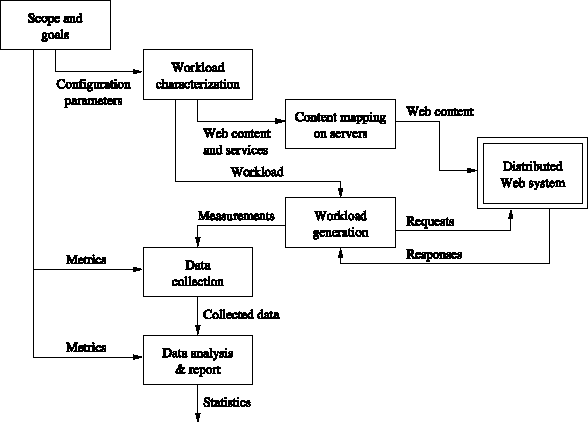
\includegraphics[width=0.8\textwidth]{benchmarking-tool-andreolini}
    \caption{Main components of a benchmarking tool for distributed Web-server systems, as per \cite{Andreolini:2002:BenchmarkingDistributedWebSystems}.}
    \label{fig:benchmarking-tool-components}
\end{figure}

The general capabilities of the ideal performance testing framework could be summarized as follows: 
\noindent
\begin{itemize} \itemsep0pt  \parsep0pt
\vspace{-\topsep}
\item Performance testing of distributed web systems.
\item \textbf{Multi-platform operation.} Support for multiple operating systems is vital, seeing that MacOS or Windows are popular in end user workstations where test scenarios are designed and debugged, while Linux-based operating systems are most frequently seen in server platforms.
\item \textbf{Architecture.} The tool should be capable of utilizing multiple machines to generate load. The architecture in terms of components would ideally resemble the system depicted in \autoref{fig:benchmarking-tool-components}.
\item \textbf{Protocols.} It should be possible to test a broad range of protocols, where the configuration should be done in a declarative manner.
\item \textbf{Modularity and extensibility.} To allow for future growth it is crucial that the framework has got a stable and rich API, which also allows for user customization for special cases, like proprietary protocols.
\item \textbf{Test types.} Stress, load, soak, others. The support should not be limited to any predefined types. Instead, through supporting proper workload modelling and injection capabilities it should be possible to configure the tool for the desired type of test.
\item \textbf{Workload definition.} Both, a declarative and an imperative approach should be available. Declarative approach might be appropriate for simple scenarios, yet a solid API is a must for more complex tests.
\item \textbf{Monitoring.} Tools for instrumentation and application and system monitoring should be a part of the framework either directly or as integrations with system tools.
\item \textbf{Reporting.} A set of tools for data processing, presentation and visualization should be provided. It should however be possible to keep raw recorded data for further processing outside of the framework.
\end{itemize}

\section{Chosen tools} \label{sec:chosen-tools}
We will analyse the capabilities and features of the tools chosen for investigation in this section. We mainly observed categories delineated in \autoref{sec:ideal-perf-test-tool}, namely architecture, protocol support, workload characterization capabilities, supported injection profiles, usability with focus on continuous integration, monitoring and reporting capabilities and finally any special features the tools might possess. The performance characteristics are further investigated in \autoref{sec:testing}.

\subsection{Faban} \label{subsec:faban}
\begin{tabularx}{\textwidth}{ ll }
  \hline
	\textbf{Tested version} & 1.3 (released 22 December 2014)  \\
	\textbf{License} 		& Apache License v2.0 \\
    \textbf{Appeared in} 	& June 2006\footnote{This is the date of the first commit in GitHub which, however, was an import from a different SCM, therefore it is very likely that Faban has appeared even earlier} \\
    \textbf{SCM} 			& \url{https://github.com/akara/faban.git} \\
    \textbf{Web} 			& \url{http://faban.org/} \\
  \hline
\end{tabularx}
\linebreak\linebreak

\noindent
Faban's website might give the untrue first impression that the project is somehow minimalistic or that it has even been abandoned. The link to the forum hosted on Google Groups\footnote{\url{https://groups.google.com/forum/\#!forum/faban-users}} proves that wrong as most community activity seems to occur there. One more peculiarity observed on the website is the warning that anyone new to Faban should ``know that there is a learning curve'' and that ``creating complex workloads does take work.'' This is in contrast to some of the other projects which try hard to sell the impression of simplicity and ease of use.

\subsection*{Architecture}
The principal modules are \textit{Faban Driver Framework} -- an API for test lifecycle control and workload definition including options for stochastic modelling of user behaviour, and \textit{Faban Harness} -- a web interface for controlling test executions (\textit{benchmark runs}). Support for running multiple driver agents is built in but not required. In case of multi-driver operation, an RMI registry first needs to be started manually on the master node. Then on each driver node, one or more agent processes are started, which in turn can run multiple agent threads, each of which hosts one \textit{driver} -- the encapsulation of a workload. The concurrency model is traditional -- one user per thread. It is possible to meticulously control the threading parameters -- a global \textit{scale} factor is declared in a test configuration and then each driver has it's \textit{threads-per-scale} configuration. Lastly, the number of agents on each node is configured. As the website warned, this complex architecture makes it slightly difficult to get to the first test run but makes it worth by offering plentiful configurability.

\subsection*{Protocols}
Faban doesn't declare much support for specific protocols, the tests need to be implemented in Java. Specific support for HTTP is provided in the form of a \texttt{HttpTransport} which features precise timing of requests and responses. For protocols with a different transport the timing is controlled manually.

\subsection*{Workload definition}
In terms of workloads Faban is again very well configurable. A test consists of multiple driver definitions, where each driver represents a single user. The ratio of drivers in a test is configurable as well. Each user can have multiple transactions (\textit{operations}) defined and there are precise controls of what order, ratio and pace the transactions are invoked in -- the transactions can be mixed according to assigned weights and think times can be chosen to fit a negative exponential distribution. These precise controls make Faban ideal for simulation of \textit{realistic} workloads.

For HTTP testing, Faban provides a supposedly simplified way to define workloads through a tool called \texttt{fhb} which consumes XML workload definitions. The vocabulary of the XML files is however just a mapping of the features provided in the Java API through annotations, therefore the usage of \texttt{fhb} is only slightly simpler since it doesn't involve compilation and packaging.

\subsection*{Injection profiles}
Timing of test runs is defined in terms of number of cycles or absolute run time. In addition to a standard flat injection profile, the ramping is configurable per test run by defining the number of cycles or time in seconds for thee parameters: ramp-up period, steady state and ramp down period. Adding to the statistical capabilities of Faban is the option to enable a uniformly distributed initial delay for driver startup, in addition to the possibility to start agents and threads all at once or sequentially. 

\subsection*{Usability}
Usability is the one point where Faban doesn't quite compare to competition and lacks in several ways. The intended entry point to Faban -- it's Harness web interface -- packs a lot of functionality that is sadly wrapped in a rather chaotic user interface. The use of the Harness is however not mandatory and all functions can be controlled otherwise. The whole test lifecycle can be controlled by manually executing runs using the master. The Harness seems to take on some functionality of a CI tool -- scheduling of runs, collection and archival of results and logs. For actual use of Faban in a CI environment, we would discourage the use of the Harness in favor of either the provided tool \texttt{fabancli} or by manually starting the master process, collecting and processing the results.

Faban doesn't seem to have any specific IDE support except for a simple guide on how to configure the NetBeans IDE for usage with Faban and how to create a project\footnote{\url{http://faban.org/1.3/docs/tutorials/netbeans.html}}.

\subsection*{Monitoring and reporting}
For internal metrics like transaction rate and response time Faban uses a very precise timer which automatically calibrates itself and accounts for the cost incurred by the timing procedures, therefore Faban should be capable of performing fine-grained microsecond-level measurements.

For system-level measurements Faban contains facilities for invocation of standard monitoring tools like \texttt{vmstat}, \texttt{iostat} and \texttt{nicstat}. The output of these tools is parsed and integrated into the reports.

\subsection*{Summary}
Faban is a very mature and powerful tool supporting the whole cycle of performance testing. It's utility is however impeded by it's complexity and difficult usage.

\subsection{Gatling} \label{subsec:gatling}
\begin{tabularx}{\textwidth}{ ll }
  \hline
	\textbf{Tested version} & 2.1.2 (released 22 December 2014)  \\
	\textbf{License} 		& Apache License v2.0 \\
    \textbf{Appeared in} 	& December 2011 \\
    \textbf{SCM} 			& \url{https://github.com/gatling/gatling.git} \\
    \textbf{Web} 			& \url{http://gatling.io} \\
  \hline
\end{tabularx}

\subsection*{Architecture}
Gatling is a simple Scala-based stress testing tool. It stands out due to it's concurrency model which is not \textit{user-per-thread} as seen in most other tools, but instead Gatling is based on Akka and Netty and makes use of an asynchronous model which depends on non-blocking implementations of transports. The number of threads needed for simulations of high numbers of virtual users is significantly lower than in user-per-thread models\footnote{The author of Gatling, St�phane Landelle, comments on the number of threads used by Gatling in this thread: \url{https://groups.google.com/forum/\#!msg/gatling/P2eYKbfygjc/P0p_prr5dlMJ}.}. The lower number of used threads also implies lower context switch rates which wastefully consume CPU resources when too many threads compete for processor time. Gatling currently doesn't have any cluster mode and runs only on a single node\footnote{There is a ``guide`` for scaling which simply states the need to execute Gatling on driver nodes manually, see \url{http://gatling.io/docs/2.1.2/cookbook/scaling_out.html}}.

\subsection*{Protocols}
Support of protocols is theoretically limited to those that have non-blocking transport implementations. Currently, Gatling supports HTTP with WebSockets and JMS out of the box. In case of JMS the final performance is inherently limited by the user-supplied JMS client implementation.

\subsection*{Workload definition}
\noindent
Gatling offers a simple DSL\footnote{Domain-specific language} for scenario definition, an example for the HTTP protocol can be seen in \autoref{lst:gatling-http-dsl}. However, writing longer scripts in this way could be tedious. For that reason, Gatling includes a ``recorder'' module in the form of an HTTP proxy which transforms captured HTTP traffic into a script of http requests, pauses and assertions about responses. That way it's possible to model the workload by either manually performing the transaction in the browser, or even capturing the traffic of another performance testing tool.

\inlinelisting
\begin{lstlisting}[label=lst:gatling-http-dsl,basicstyle=\ttfamily, showstringspaces=false, language=Java, caption={Gatling's DSL for HTTP requests}]
http("Open product page")
  .get("https://www.example.com/products")
  .queryParam("product", "123")
  .check(status.is(200))
\end{lstlisting}

The Gatling DSL offers various elements that can be combined to construct a workload. Transactions are defined as chains of these elements, such as protocol operations like \texttt{http.get(...)}, structural elements like loops and switches, pauses and others. The workloads can be parameterized using the facility of \textit{feeders}, which are functions capable of generating or loading data from various sources and exposing them as variables usable in the transaction script.

\subsection*{Injection profiles}
Each defined transaction can have a separate injection profile. Just like the workload, the profile is constructed from language elements, such as \texttt{nothingFor(duration)} for a pause, \texttt{atOnceUsers(number)} for an immediate injection, \texttt{rampUsers(number) over (duration)} for a linear ramp-up, and continuous variants of the two mentioned elements -- \texttt{constantUsersPerSec(number)} and \texttt{rampUsersPerSec(number)} and several others. These elements can be combined to form complex profiles.

\subsection*{Usability}
The fastest way to stress testing awaits those who already know Scala. However, for most use cases no significant knowledge of the language is required as the DSL is easily comprehensible and the scenarios are basically self-documenting. A strong point to Gatling is the documentation which besides clearly communicating the intended usage of the application also serves in some parts as a best practices guide for performance testing in general. 

One minor complication for a user experienced in using other performance testing tools with traditional threading approach might be the slight conceptual difference in understanding what an \textit{active user} means. Traditionally, one thread performs cyclically the operations of one virtual user. In Gatling, \textit{injecting a user} means initiating the user transaction and that user is considered \textit{active} until the end of that one \textit{transaction}. 
 
\subsection*{Monitoring and reporting}
An HTML report with statistics of throughput and response times in tabular form and in the form of interactive charts is automatically generated from a test run. Response time statistics include percentiles, maximum, mean and standard deviation. The charts show throughput and response time as a function of time and a response time distribution plot. All these statistics are also broken down by individual operations. Overall, the report is very comprehensible. Gatling does not provide any facility for monitoring system resources.

\subsection*{Summary}
Gatling is a tool best suited for testing web application throughput and responsiveness through HTTP. It appears to be targeted at agile development methodologies due to its conceptual simplicity, gentle learning curve and straightforward setup and execution.
 
\subsection{Grinder} \label{subsec:grinder}
\begin{tabularx}{\textwidth}{ ll }
  \hline
	\textbf{Tested version} & 3.11 (released 25 October 2012)  \\
	\textbf{License} 		& BSD License (modified) \\
    \textbf{Appeared in} 	& December 2000 \\
    \textbf{SCM} 			& \url{http://git.code.sf.net/p/grinder/code} \\
    \textbf{Web} 			& \url{http://grinder.sourceforge.net/} \\
  \hline
\end{tabularx}
\linebreak\linebreak

\noindent

\subsection*{Architecture}
Grinder is a JVM-based tool which primarily supports scripting in Jython and recently also Clojure. Clustered operation is supported by default and agents can even execute test without the master \textit{console}. Multiple agent processes can run on each machine and each agent process executes worker threads for tests. Terminology in Grinder is used slightly atypically -- the top-level element for Grinder is a \textit{script} which instantiates \texttt{Test} objects which record metrics. 

\subsection*{Protocols}
Support for many protocols is declared in the documentation, however, the ``support'' is only in the form of standard Java APIs. The only specific support is for the HTTP protocol using a plugin, which provides additional statistics like mean response length, mean time to resolve host or mean time to establish connection.

\subsection*{Workload definition}
The work of defining virtual user behaviour is again left almost completely to the test developer without much support for stochastic modelling -- the maximum sleep time before script execution and its variation are configurable, though their normal distribution is not. The suggested way of executing multiple scenarios with different weights is instantiating other scripts from the running script based on the result of the modulo function applied to the current thread ID\footnote{\url{http://sourceforge.net/p/grinder/code/ci/master/tree/grinder/examples/proportion.py}}. There exists, at least, the option to record a transaction using Grinder's TCPProxy which, similarly to Gatling's recorder, captures network traffic into a format consumable by Grinder.

\subsection*{Injection profiles}
There does not seem to be any support for injection profiles, except for another provided example which suggests invoking a sleep for the duration defined as thread index multiplied by a number of milliseconds.

\subsection*{Usability}
Grinder features a Java Swing GUI and a REST endpoint. Both interfaces support similar set of features which includes: managing lifecycle of workers, distribution of test scripts to workers and access to recorded data. The REST endpoint makes Grinder well suitable for a CI environment.

\subsection*{Monitoring and reporting}
Measurements in Grinder are performed -- unlike in any of the other tools -- exclusively through instrumentation. This method directly manipulates bytecode in memory and inserts measurement procedures. The advantage to this approach is its simplicity and flexibility -- it allows the user to instrument any piece of code and measure the execution time of methods, as demonstrated in \autoref{lst:grinder-test-instrumentation}. This approach seems inevitable given that the user needs to implement all of the protocol support himself. The provided HTTP plugin is instrumented implicitly. 

\noindent
\begin{minipage}{\linewidth}
\inlinelisting
\begin{lstlisting}[label=lst:grinder-test-instrumentation,basicstyle=\ttfamily, showstringspaces=false, language=Python, caption={Grinder's test instrumentation}]
test1 = Test(1, "Service test")
service = SomeService()

# Instrument all calls to service
test1.record(service)
  
class TestRunner:
    def __call__(self):
        service.call("Instrumentation test")
\end{lstlisting}
\end{minipage}

\noindent
The collected data is output to two files: a summary log file which contains aggregated statistics for all tests and their metrics and a second file containing raw measurement data for \textit{every} request-response pair. This is rather inconvenient as this data has not much value in itself and needs to be further processed, aside from the fact that the file size can reach hundreds of megabytes even for short tests. Live data during a test run can be seen in the graphical console, which however doesn't provide much value in a CI environment. There is a separate tool for analysis of raw Grinder data into PNG files\footnote{\url{http://track.sourceforge.net/}}.

\subsection*{Summary}
Put simply, Grinder is a DIY sort of tool, whereby many of its declared features rely on external tools and the user's capability to handle aspects of performance testing by writing their own Python or Java code for the purpose. Therefore Grinder is only as powerful as is its user.

\subsection{JMeter} \label{subsec:jmeter}
\begin{tabularx}{\textwidth}{ ll }
  \hline
	\textbf{Tested version} & 2.12 (released 9 November 2014)  \\
	\textbf{License} 		& Apache License v2.0 \\
    \textbf{Appeared in} 	& September 1998 \\
    \textbf{SCM} 			& \url{http://svn.apache.org/repos/asf/jmeter/trunk} \\
    \textbf{Web} 			& \url{http://jmeter.apache.org/} \\
  \hline
\end{tabularx}
\linebreak\linebreak

\subsection*{Architecture}
JMeter has probably been around the longest time among the reviewed tools and it's apparent in its exceptionally broad feature set. 
It supports clustered testing in the usual way, however, with slightly unusual terminology -- the process executed on the driver which is usually called an \textit{agent} is called, somewhat confusingly, a JMeter \textit{server}. The complementary part residing on the coordinating node is called, as expected, the \textit{client}. The main building blocks of JMeter's model are: the top-level \textit{ThreadGroup} which holds all other elements, \textit{samplers} which generate the load and \textit{listeners} which gather measurement data.

\subsection*{Protocols}
The list of supported protocols is similarly broad as the feature set. This includes HTTP, FTP, JDBC, SOAP, LDAP, JMS, SMTP and more. In this case, as opposed to e.g. Grinder, the protocols are \textit{actually} supported in the sense that the user doesn't need to know or use any APIs, all protocols are accessed declaratively.

\subsection*{Workload definition}
The test plans are stored in markedly verbose XML files. On the positive side, they are still somewhat human-readable and can therefore be checked in to an SCM and compared using \texttt{diff}. On the other hand, they are clearly not \textit{intended} to be read by humans, as seen in \autoref{lst:jmeter-xml-verbosity}. JMeter has a rich GUI whose strongest side is creation of test plans. It can as well be used to run the tests but is not required for that purpose.

The actual workload definition is composed of \textit{samplers} which generate load, \textit{logic controllers} which build up the structure of the transaction using switches, loops, conditions, randomization or interleaving, and finally \textit{timers} which allow for some statistical modelling using uniform, Gaussian or Poisson distributions of the timed operations.

\noindent
\begin{minipage}{\linewidth}
\inlinelisting
\begin{lstlisting}[label=lst:jmeter-xml-verbosity,basicstyle=\ttfamily, breaklines=true, showstringspaces=false, language=XML, caption={JMeter's verbose XML configuration}]
<ThreadGroup guiclass="ThreadGroupGui" testclass="ThreadGroup" testname="HTTP GET" enabled="true">
  <stringProp name="ThreadGroup.on_sample_error">stoptest</stringProp>
  <elementProp name="ThreadGroup.main_controller" elementType="LoopController" guiclass="LoopControlPanel" testclass="LoopController" testname="Loop Controller" enabled="true">
    <boolProp name="LoopController.continue_forever">false</boolProp>
    <intProp name="LoopController.loops">-1</intProp>
  </elementProp>
  <stringProp name="ThreadGroup.num_threads">32
  </stringProp>
  <stringProp name="ThreadGroup.ramp_time">0
  </stringProp>
    ...
\end{lstlisting}
\end{minipage}

\subsection*{Injection profiles}
JMeter only seems to support a linear ramp-up profile, in addition to a flat big-bang profile. However, owing to JMeter's extensibility through plugins, other features including new injection profiles can be supported, like a stepped ramp-up profile\footnote{\url{http://jmeter-plugins.org/wiki/SteppingThreadGroup/}}. 

\subsection*{Usability}
JMeter has a gentle learning curve thanks to its powerful GUI, which is JMeter's blessing and a curse -- it is very intuitive and easy to use, however, it's the only reasonable way of defining test plans. It's possible to execute JMeter in a headless mode, have it manage the test run on driver nodes and exit after the test run. 

\subsection*{Monitoring and reporting}
Measurements are gathered using \textit{listeners}, some of which are intended primarily for visualization in the GUI while others generate tabular summaries, aggregate statistics and sample distributions. All of the expected measurements and metrics are present including latency, response time, response size, throughput and their minima, maxima, mean and median. JMeter doesn't have a facility for monitoring performance data built in, but again, there's a plugin for that\footnote{\url{http://jmeter-plugins.org/wiki/PerfMon/}}.

\subsection*{Summary}
JMeter is among the most powerful tools we have reviewed and seems to be one of the most capable in all categories.

\subsection{PerfCake} \label{subsec:perfcake}
\begin{tabularx}{\textwidth}{ ll }
  \hline
	\textbf{Tested version} & 3.3 (released 21 October 2014)  \\
	\textbf{License} 		& Apache License v2.0 \\
    \textbf{Appeared in} 	& April 2013 \\
    \textbf{SCM} 			& \url{https://github.com/PerfCake/PerfCake} \\
    \textbf{Web} 			& \url{https://www.perfcake.org/} \\
  \hline
\end{tabularx}
\linebreak\linebreak

\subsection*{Architecture}
PerfCake is the youngest project we have reviewed, having appeared less than two years ago. The top-level element is called a \textit{scenario} and its key sub-elements are: a \textit{generator} which defines the injection profile, a \textit{sender} which defines the target and the protocol. The concurrency model is the standard thread-per-user model which, however, seems to be implemented more efficiently compared to other tools by maintaining a \textit{queue} of threads that take turns sending messages. PerfCake currently does not support multi-node operation but it seems to be on the roadmap\footnote{\textit{Add support for running PerfCake in cluster}, open issue on Github, \url{https://github.com/PerfCake/PerfCake/issues/44}}.

\subsection*{Protocols}
Several protocols are supported: HTTP, JDBC, JMS, LDAP, plain socket, WebSockets, all available as senders.

\subsection*{Workload definition}
PerfCake doesn't seem to have much support for workload definition currently. The only way to specify a sequential scenario is by declaring multiple messages which will then be sent in a round-robin fashion by the declared sender without any control structures or options for timing. There is a way to perform custom operations in a transactions in an out-of-band fashion by using the \texttt{CommandSender} or \texttt{GroovySender} to invoke any system command or a groovy script, respectively. That however, has the significant drawback of stepping outside of the PerfCake process and thus losing proper measurement support and obviously, the significant overhead of process creation.

\subsection*{Injection profiles}
Generators are responsible for defining the injection profile. The \texttt{Default\allowbreak{}Message\allowbreak{}Generator} corresponds to a flat profile and the \texttt{Ramp\allowbreak{}Up\allowbreak{}Down\allowbreak{}Generator} does just what it says -- supports a linear ramping profile consisting of a initial flat, ramp-up, main flat, ramp-down and final flat phases.

\subsection*{Usability}
The XML format used for scenario declaration is easily comprehensible as it is apparently meant to be written by hand. However, plugins for the Eclipse and IDEA development environments are already available and allow visual design of scenarios and test execution from the IDE. One strange issue is the current state of PerfCake's documentation. Quite understandably, it is still unfinished. However, the fact that it's only available in PDF format makes it much less accessible.

\subsection*{Monitoring and reporting}
This seems to be a strong aspect of PerfCake, or promising at least. Even though PerfCake doesn't currently generate any visual output, it does feature certain clever \textit{reporters}. One of them is the \texttt{WarmUpReporter} which applies regression analysis to the response time values and indicates whether the system doesn't show too much jitter in the measurement and is therefore likely to be warmed up. Another clever analysis tool is the \texttt{MemoryUsageReporter} which is capable of analysing the slope of the trend of used memory and indicate a possible memory leak.

\subsection*{Summary}
PerfCake is apparently in its early stages and seems to be just gaining traction and finding its user base, but showing promise with clever features not commonly seen elsewhere. It manifests some bugs in recently designed features which just hadn't had the chance to be caught yet, but were fixed promptly. Conceptually, PerfCake is very simple or even simplistic and it will be interesting to see how to will accommodate future additions of features. 

\section{Other tools} \label{sec:other-tools}
We would like to mention several other performance testing tools which for various reasons weren't chosen for investigation in these thesis but are definitely worth mentioning, for the sake of completeness:
\begin{itemize} \itemsep0pt  \parsep0pt
\vspace{-\topsep}
\item \textbf{Tsung}\footnote{\url{http://tsung.erlang-projects.org/}} was not chosen as it is not a JVM-based tool, is written in Erlang and doesn't support some of the required protocols. It focuses on realistic modelling of web traffic using a stochastic model developed as part of a research \cite{Liu:2001:TMP:570289.570291}.
\item \textbf{jmh}\footnote{\url{http://openjdk.java.net/projects/code-tools/jmh/}} is not targeted at web applications, but instead, it is a tool for microbenchmarks in the JVM
\item \textbf{RadarGun}\footnote{\url{https://github.com/radargun/radargun/}} specializes in testing distributed caches and data grids and appears to be a well established tool with a broad feature set
\end{itemize}

\section{Comparison} \label{sec:tools-comparison}
The following table summarizes the subjective evaluation from \autoref{sec:chosen-tools}. Each tool is assigned points in each category from 0 meaning the support for that aspect is non-existent or significantly broken or insufficient, up to 4 meaning the tool fulfils or surpasses expectations in that aspect.\\

\noindent
\begin{tabular}{ |p{3cm}|c|c|c|c|c| }
\hline
							& Faban & Gatling & Grinder & JMeter & PerfCake \\
\hline
Architecture				& $\bullet$$\bullet$$\bullet$ & $\bullet$$\bullet$$\bullet$ & $\bullet$$\bullet$$\bullet$ & $\bullet$$\bullet$$\bullet$$\bullet$ & $\bullet$$\bullet$ \\
\hline
Protocols					& $\bullet$ & $\bullet$$\bullet$ & $\bullet$ & $\bullet$$\bullet$$\bullet$$\bullet$ & $\bullet$$\bullet$$\bullet$ \\
\hline
Workload definition			& $\bullet$$\bullet$$\bullet$$\bullet$ & $\bullet$$\bullet$$\bullet$$\bullet$ & $\bullet$ & $\bullet$$\bullet$$\bullet$$\bullet$ & $\bullet$ \\
\hline
Injection profiles			& $\bullet$$\bullet$$\bullet$ & $\bullet$$\bullet$$\bullet$$\bullet$ & & $\bullet$$\bullet$ & $\bullet$$\bullet$$\bullet$ \\
\hline
Usability					& $\bullet$ & $\bullet$$\bullet$$\bullet$ & $\bullet$$\bullet$$\bullet$ & $\bullet$$\bullet$$\bullet$$\bullet$ & $\bullet$$\bullet$$\bullet$$\bullet$ \\
\hline
Monitoring and reporting	& $\bullet$$\bullet$$\bullet$ & $\bullet$$\bullet$$\bullet$ & $\bullet$$\bullet$$\bullet$ & $\bullet$$\bullet$$\bullet$ & $\bullet$$\bullet$$\bullet$ \\
\hline
\end{tabular}


\section{Discussion}
Most of the tools evaluated are very well suitable for performance testing of web applications and our final recommendations based on the evaluation would be as follows:
\begin{itemize} \itemsep0pt  \parsep0pt
\vspace{-\topsep}
\item JMeter for cases where testing of many protocols and complex scenarios is required,
\item Gatling for a start-up company which requires fast turnaround,
\item Faban perhaps for large enterprises which need a stable tool and can invest the necessary time for learning and deployment,
\item PerfCake seems to be the best for testing software in active development, possessing unique features for bug discovery,
\item Grinder, despite falling behind in most categories, is still a valuable tool which offers a great degree of flexibility and scripting capability.
\end{itemize}

%
%%%%%%%%%%%%%%%%%%%%%
%
%    CHAPTER: Testing tools put to the test
%
%%%%%%%%%%%%%%%%%%%%%
%

\chapter{Testing tools put to the test} \label{chap:testing-the-tools}
The performance characteristics of all the tools described earlier in \autoref{sec:chosen-tools} are compared in this chapter. Only a small subset of capabilities shared by all the tools was chosen for deeper investigation. We focused on testing of four protocols: HTTP, REST\footnote{Notwithstanding the original definition of REST as an \textit{architectural style}\cite{Fielding:2002:PDM:REST}, it is commonly referred to as a \textit{protocol}, perhaps due to its role being similar to that of standards such as SOAP, which is a protocol indeed.}, JMS and SOAP, with a single load-generating node against a single server node. The \hyperref[subsec:scenarios]{scenarios}, \hyperref[subsec:server-configuration]{application server configuration}, and the \hyperref[subsec:sample-app]{sample application} used for testing are described in more detail in \autoref{sec:methodology}. 

\section{Environment}\label{sec:environment}
The environment used for testing was chosen so as to emulate the real world conditions in which large scale web applications are executed, in terms of hardware performance, architecture and operating system. Two different machines were used for testing -- a \textit{server} and a \textit{driver}. The server machine hosts the application server and all other server-side resources required for the operation of the application server. The driver machine runs the performance testing software and all its load generation processes. One more machine was used for auxiliary functions, mainly coordination. We will call it the \textit{master}. 

There are several considerations that had to be taken into account when setting up the environment for testing, the most important being a good balance between performance of the driver and the server. Generally, to obtain reasonable results in performance testing, the driver machine hardware needs to be sufficiently powerful to simulate the load normally coming from many distributed users working with the application. The total throughput capacity of requests generated by the load-generating node must surpass the maximum throughput the server is capable of processing. For this reason, the load generation is often distributed to multiple machines also in testing. 

However, in our case, we chose performance characteristics \textit{inverse} to the ones described above -- the hardware of the server machine is slightly \textit{more} powerful than the driver hardware. Our intention was to keep the resource utilization of the server machine reasonably below the upper extremes and to compare the load generation capability of the tested software at the maximum resource utilization of the driver machine, without being limited by the server side.

\noindent
The server machine:
\begin{itemize} \itemsep0pt  \parsep0pt
\vspace{-\topsep}
\item dedicated physical machine
\item RHEL 6.5 Server x86\_64 operating system
\item two 4-core 2.5 GHz Intel Xeon processors, 8 cores total
\item 48 GB of DDR2 RAM
\end{itemize}

\noindent
The driver machine:
\begin{itemize} \itemsep0pt  \parsep0pt
\vspace{-\topsep}
\item dedicated physical machine
\item RHEL 6.5 Server x86\_64 operating system
\item two 4-core 2.13 GHz Intel Xeon processors, manually restricted to 4 online cores
\item 24 GB of DDR3 RAM
\end{itemize}

\noindent
The master machine:
\begin{itemize} \itemsep0pt  \parsep0pt
\vspace{-\topsep}
\item dedicated physical machine
\item RHEL 6.5 Server x86\_64 operating system
\item single 4-core 2.0 GHz Intel Xeon processor, 4 cores total
\item 6 GB of DDR3 RAM
\end{itemize}

\noindent
\\
The two main machines -- server and driver -- were interconnected through a 1 Gbit/s Ethernet link without any intermediate network nodes, possibly a switch. To make sure that the network environment was sane and was not a limiting factor, the network latency and throughput were verified several times throughout testing. The \texttt{ping} command indicated an average packet round-trip time of 0.2 ms. The throughput was measured using the iperf\footnote{\url{http://iperf.sourceforge.net}} software. The iperf tool was configured to transfer TCP data from client to server for 20 seconds in 20 parallel connections, and this test was performed in both directions, using the command shown in \autoref{lst:iperf-throughput}. The transfer rate averaged at 935 Mbit/s in both directions, which we consider a satisfactory result in light of the practical data rate limit of common Gigabit Ethernet hardware which, in ideal conditions, appears to be at 987 MBit/s. \footnote{LAN Ethernet Maximum Rates, Generation, Capturing \& Monitoring, from \url{http://wiki.networksecuritytoolkit.org/nstwiki/index.php/LAN_Ethernet_Maximum_Rates,_Generation,_Capturing_\%26_Monitoring}}

\inlinelisting
\begin{lstlisting}[label=lst:iperf-throughput,basicstyle=\ttfamily, language=bash, caption={network throughput test}]
iperf -c <server_address> -P 20 -t 20 -i 1
\end{lstlisting}

Coordination of test runs was facilitated by Jenkins\footnote{Jenkins is web-based continuous integration software, see \url{http://jenkins-ci.org}.} running in an internal instance of OpenShift\footnote{OpenShift is a PaaS service, see \url{http://openshift.com}.}, which had a 100 MBit/s link to the three testing machines, master, server and driver, all of which were registered as Jenkins slaves and thus easily controllable from a single point. Automation of test runs simplifies reproduction of results. Configurations of all test jobs and all necessary scripts are available on the attached medium.

The version of Java used on all nodes was OpenJDK 1.7.0\_71.

\section{Methodology} \label{sec:methodology}
We applied the following general rules during all tests:
\begin{itemize} \itemsep0pt  \parsep0pt 
\vspace{-\topsep}
	\item \textbf{Distributed mode.} Whenever the tool provided a mode for clustered testing we tried to apply that by running the controller process on the master machine and the agent process on the driver machine. This provided the most resources for the driver without being limited by resource usage of the controller process.
	\item \textbf{Monitoring.} We monitored the system resources on the driver and the server using the \texttt{dstat}\footnote{\textit{dstat: Versatile resource statistics tool}, \url{http://dag.wiee.rs/home-made/dstat/}} tool to have a reference point for investigation of possible problems and for cases where the measurements could correlate to system resources.
\end{itemize}

All tests were executed 3 times to ensure reliability of results. The results indicated in the tables of results for each tool are averages from all samples of all 3 runs. The unit of measurement is ``operations per second''.

\subsection{Server configuration} \label{subsec:server-configuration}
A JBoss Enterprise Application Platform (EAP) 6.3.0 server was used for all testing. EAP is the product variant of the freely available JBoss AS which now known as WildFly. EAP is an application server which fully implements the Java EE 6 standard.
The server was started from an unzipped distribution before each test execution. The server was executed using the \texttt{standalone-full} configuration which enabled all required subsystems including messaging. We did not apply any specific configuration to the server except for necessary adjustments and one minor tweak:
\begin{itemize} \itemsep0pt  \parsep0pt 
\vspace{-\topsep}
	\item the server was bound to all available network interfaces, to the address 0.0.0.0
	\item one application user was configured for authentication in protocols which required it
	\item journal persistence of the messaging subsystem was disabled due to problems encountered in one of the tests
\end{itemize}

\subsection{Sample application} \label{subsec:sample-app}
The application used for testing was a minimalistic implementation of the tested protocols. The only response it provided to a request in each protocol was a fixed message no longer than several bytes. The listeners for each protocol were implemented as follows:
\begin{itemize} \itemsep0pt  \parsep0pt 
\vspace{-\topsep}
	\item \textbf{HTTP} by a Servlet,
	\item \textbf{JMS} by a Message-driven bean listening on one queue and sending responses to another, setting the correlation ID of the response to the message ID of the receive message,
	\item \textbf{REST} using the JAX-RS API by an endpoint responding to \texttt{GET} requests with a \texttt{text/plain} media type,
	\item \textbf{WS-SOAP} using the JAX-WS API by a web service endpoint with one method.
\end{itemize}

\subsection{Scenarios} \label{subsec:scenarios}
 The following common conditions applied to all scenarios:

\begin{itemize} \itemsep0pt \parsep0pt 
\vspace{-\topsep}
	\item 10 minutes execution time;
	\item no think time between requests;
	\item optional warm up, only used if the tool supports it and does not include the warm up period in results;
	\item the number of threads or virtual users was manually adjusted to a reasonable value at which the tool would use the most processor time and beyond which the number of transactions per second didn't seem to improve;
	\item use the native support for a protocol whenever available, implement a substitute solution otherwise;
	\item use keep-alive connections for transports where available.
\end{itemize}

\noindent
These individual scenarios were executed for each tool:
\begin{itemize} \itemsep0pt \parsep0pt 
\vspace{-\topsep}
	\item \textbf{HTTP}: single GET request,
	\item \textbf{REST}: single GET request,
	\item \textbf{JMS}: request-response -- send a 5-byte long request to one queue and receive a response from another; use asynchronous communication using a listener where available,
	\item \textbf{WS-SOAP}: invoke one web service method using the way recommended or most straightforward in a given tool -- either manually POST an XML document over HTTP, or use a client generated using the \texttt{wsimport}\footnote{\url{http://docs.oracle.com/javase/6/docs/technotes/tools/share/wsimport.html}} tool when more appropriate.
\end{itemize}

\section{Testing} \label{sec:testing}
This section will describe the implementation of the scenarios in each individual tool, possible problems which were encountered during testing and the results of measurements.

The first issue that was encountered in preliminary testing was the imbalance between performance of the client and the server. More precisely, both machines were similarly equipped in terms of CPU, however, with all 8 cores enabled on the driver, the load imposed on the server was too high and the server's resources were exhausted faster than on the driver. For this reason the number of cores on the driver was halved to 4 cores. This was done using the \texttt{sysfs} facility available in Linux, by issuing the command shown in \autoref{lst:sysfs-disable-cores} analogously for cores 4--7:

\noindent
\begin{minipage}{\linewidth}
\inlinelisting
\begin{lstlisting}[label=lst:sysfs-disable-cores,basicstyle=\ttfamily, breaklines=true, showstringspaces=false, language=bash, caption={Disabling CPU cores on a live system}]
$> echo 0 > /sys/devices/system/cpu/cpu4/online
\end{lstlisting}
\end{minipage}

\noindent
The client used in JMS tests was a HornetQ JMS Client version 2.3.20\footnote{\url{https://github.com/hornetq/hornetq/tree/HornetQ_2_3_20_Final}} which corresponded to the version of HornetQ Server in JBoss EAP 6.3.0.

\pagebreak[4]
\subsection{Faban}
Each Faban benchmark was executed in a distributed configuration with one master and one client. The injection profile was always: 60 seconds ramp-up before the test, 10 minutes of steady state at maximum load and 30 seconds of ramp-down afterwards.

\begin{figure}[h]
    \centering
    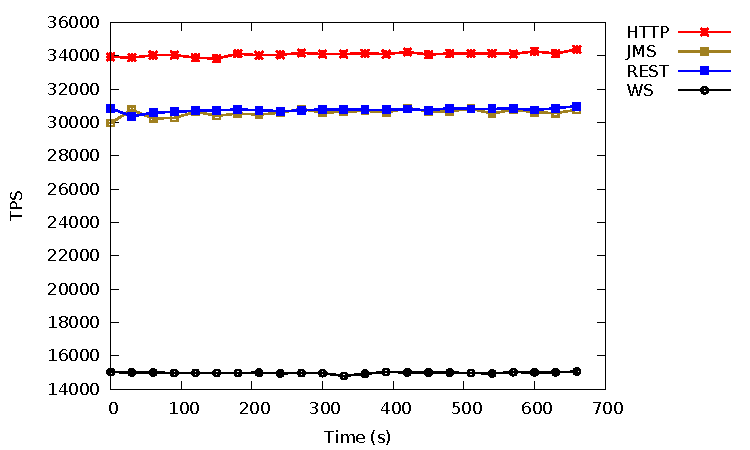
\includegraphics[width=0.8\textwidth]{faban-tps}
    \caption{Faban throughput}
    \label{fig:faban-throughput}
\end{figure}

For the HTTP test there was the possibility to use Faban's simplified HTTP driver \texttt{fhb} which we opted not to use since it very likely wouldn't provide any difference in performance and all the other drivers were implemented using the Java API, so the HTTP test used it as well.

Faban doesn't provide any specific support for the JMS protocol, therefore we considered it officially unsupported, but decided to try implementing an asynchronous JMS driver anyway, inspired by the design used in JMeter's JMS sampler\footnote{\url{https://github.com/apache/jmeter/tree/trunk/src/protocol/jms/org/apache/jmeter/protocol/jms/sampler}}.

For the SOAP test, the \texttt{wsimport}-generated client was used.

\begin{center}
\begin{tabularx}{0.7\textwidth}{ |X|X| }
	\hline
	\multicolumn{2}{|c|}{Faban results} \\
	\hline
	HTTP 	& 34088 op/s \\
	\hline
	JMS 	& 30581 op/s \\
	\hline
    REST 	& 30748 op/s \\
    \hline
    SOAP 	& 14974 op/s \\
  \hline
\end{tabularx}
\end{center}

\pagebreak[4]
\subsection{Gatling}
Gatling posed a couple of problems which needed to be resolved before proper testing. One problem appeared when Gatling couldn't execute high numbers of concurrent users due to a system limit on open files. This problem was found to be described in the documentation\footnote{\url{http://gatling.io/docs/2.1.2/general/operations.html}} and the open file limit was raised to 300000.

\begin{figure}[h]
    \centering
    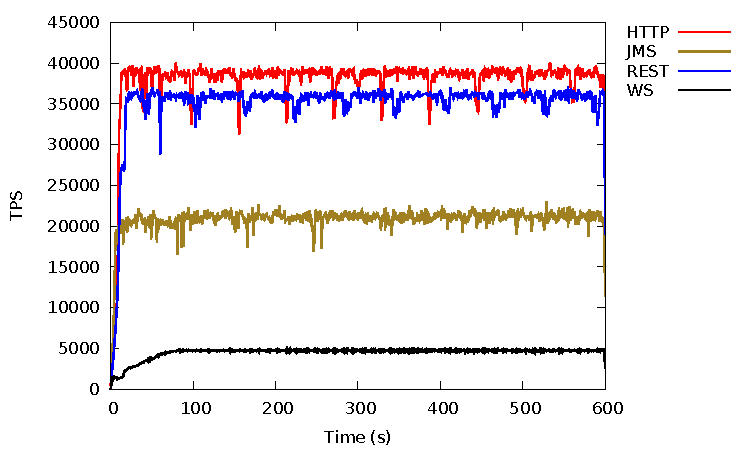
\includegraphics[width=0.8\textwidth]{gatling-tps}
    \caption{Gatling throughput}
    \label{fig:gatling-throughput}
\end{figure}

Another problem stemmed from Gatling's concurrency model and the use of asynchronous HTTP client: certain virtual users spent in Gatling's message queue apparently longer than 60 seconds and connections started timing out. This was remedied by increasing connection and read timeouts in Gatling's configuration.

For the SOAP test the approach of sending an XML file through the HTTP protocol was used since Gatling doesn't have any particular support for SOAP.

\begin{center}
\begin{tabularx}{0.7\textwidth}{ |X|X| }
	\hline
	\multicolumn{2}{|c|}{Gatling results} \\
	\hline
	HTTP 	& 37872 op/s \\
	\hline
	JMS 	& 20822 op/s \\
	\hline
    REST 	& 35096 op/s \\
    \hline
    SOAP 	& 4504 op/s \\
  \hline
\end{tabularx}
\end{center}

\pagebreak[4]
\subsection{Grinder}
Grinder posed another unforeseen obstacle: by keeping too many connections open at the same time, an exception started appearing: \texttt{java.\allowbreak{}net.\allowbreak{}NoRouteToHostException: Cannot assign requested address}. We found the ultimate reason was exhaustion of the pool of available ephemeral ports. The solution we decided to apply was allowing the system to reuse connections in the \texttt{TIME\_WAIT} state by issuing the command in \autoref{lst:sysfs-tcp-rw-reuse}.

\noindent
\begin{minipage}{\linewidth}
\inlinelisting
\begin{lstlisting}[label=lst:sysfs-tcp-rw-reuse,basicstyle=\ttfamily, breaklines=true, showstringspaces=false, language=bash, caption={Allow the reuse of unclosed connections}]
$> echo 1 > /proc/sys/net/ipv4/tcp_tw_reuse
\end{lstlisting}
\end{minipage}

For the SOAP test we used the generated WS client. JMS is not supported and in this case instead of a custom JMS driver we chose to try using synchronous mode with correlation of messages using a selector on the response queue.

\begin{figure}[h]
    \centering
    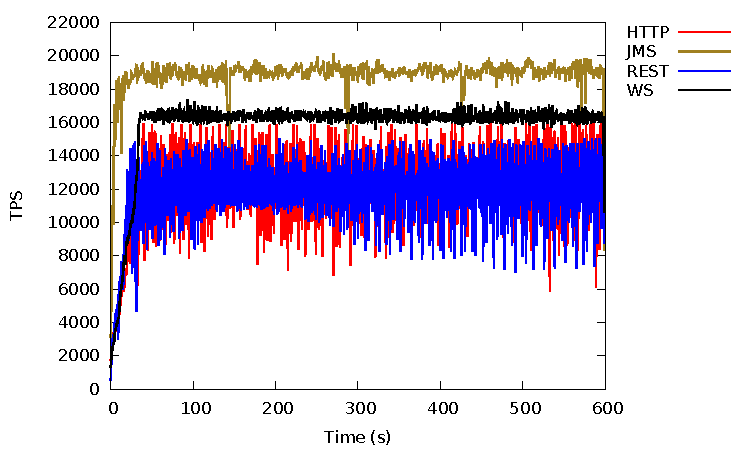
\includegraphics[width=0.8\textwidth]{grinder-tps}
    \caption{Grinder throughput}
    \label{fig:grinder-throughput}
\end{figure}

\begin{center}
\begin{tabularx}{0.7\textwidth}{ |X|X| }
	\hline
	\multicolumn{2}{|c|}{Grinder results} \\
	\hline
	HTTP 	& 12189 op/s \\
	\hline
	JMS 	& 18866 op/s \\
	\hline
    REST 	& 11829 op/s \\
    \hline
    SOAP 	& 15845 op/s \\
  \hline
\end{tabularx}
\end{center}

\pagebreak[4]
\subsection{JMeter}
All tested protocols are explicitly supported by JMeter, therefore no custom client was required. One issue appeared which has not been resolved despite all attempts: 0.03\% of transactions in the JMS test were erroneous.

\begin{figure}[h]
    \centering
    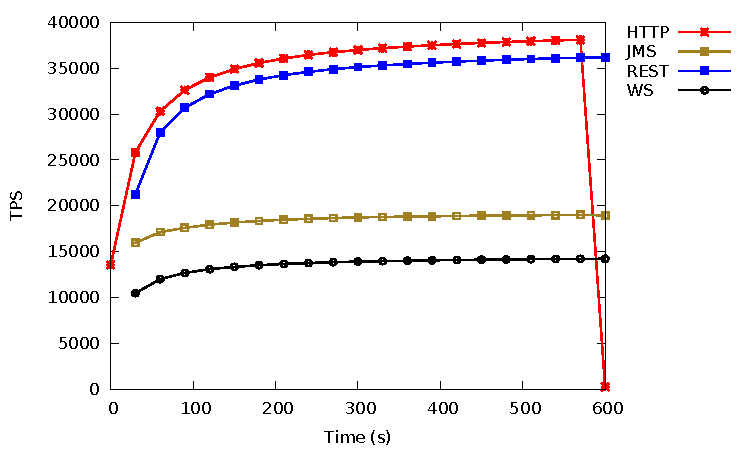
\includegraphics[width=0.8\textwidth]{jmeter-tps}
    \caption{JMeter throughput}
    \label{fig:jmeter-throughput}
\end{figure}

\begin{center}
\begin{tabularx}{0.7\textwidth}{ |X|X| }
	\hline
	\multicolumn{2}{|c|}{JMeter results} \\
	\hline
	HTTP 	& 34622 op/s \\
	\hline
	JMS 	& 18429 op/s \\
	\hline
    REST 	& 33807 op/s \\
    \hline
    SOAP 	& 13565 op/s \\
  \hline
\end{tabularx}
\end{center}

\pagebreak[4]
\subsection{PerfCake}
No significant issues appeared while testing PerfCake. Support for JMS is integrated and the SOAP test was implemented through the \texttt{HttpSender}.

\begin{figure}[h]
    \centering
    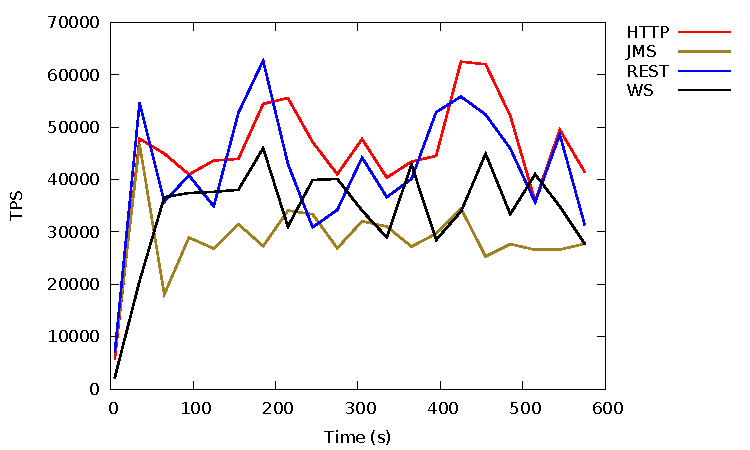
\includegraphics[width=0.8\textwidth]{perfcake-tps}
    \caption{PerfCake throughput}
    \label{fig:perfcake-throughput}
\end{figure}

\begin{center}
\begin{tabularx}{0.7\textwidth}{ |X|X| }
	\hline
	\multicolumn{2}{|c|}{PerfCake results} \\
	\hline
	HTTP 	& 45751 op/s \\
	\hline
	JMS 	& 28126 op/s \\
	\hline
    REST 	& 44568 op/s \\
    \hline
    SOAP 	& 33363 op/s \\
  \hline
\end{tabularx}
\end{center}

\pagebreak[4]

\section{Results}

The tool with the highest throughput in HTTP appears to be PerfCake with over 45000 op/s, as shown in \autoref{fig:http-summary}. The profile of PerfCake is very bursty but still higher on average. It should be noted that the granularity of reporting was not equal for all tools and that might cause differences in the curves, possibly increasing the burstiness with higher precision of measurement.

\begin{figure}[h]
    \centering
    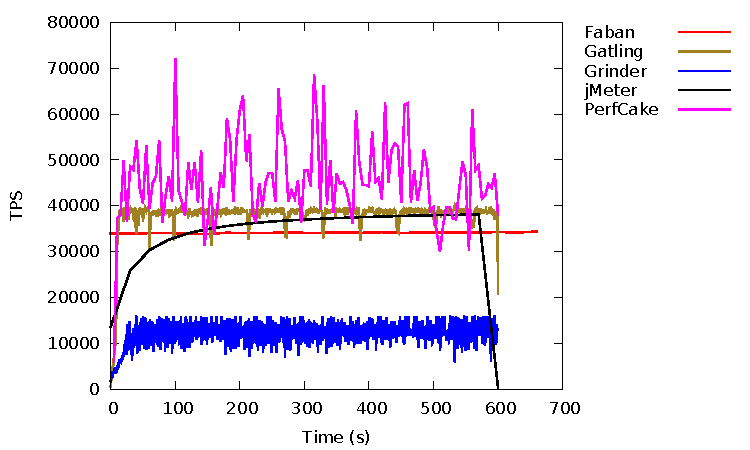
\includegraphics[width=0.8\textwidth]{http-summary}
    \caption{HTTP summary}
    \label{fig:http-summary}
\end{figure}

The JMS test was especially tricky since not all the tools had native support for the protocol. Additionally, all of the JMS tests depended on the HornetQ driver implementation which might have been a limiting factor. This theory is supported by the data showing that there's the least variance between tools in the JMS test compared to other tests, as seen in \autoref{fig:jms-summary}.

\begin{figure}[h]
    \centering
    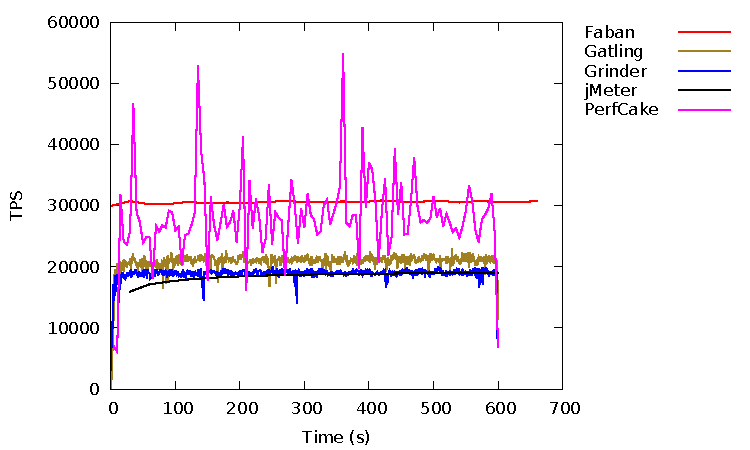
\includegraphics[width=0.8\textwidth]{jms-summary}
    \caption{JMS summary}
    \label{fig:jms-summary}
\end{figure}

The HTTP and REST tests were expected to yield very similar results in each individual tool, since the transport for both is HTTP and they used the same method and all other parameters. REST was therefore considered more of a ``control sample''. This expectation turned out to be mostly true, with REST performing very slightly less in each tool despite the great similarity to HTTP. The reasons behind this could possibly include a little longer response time with REST, since the request needs to traverse a longer processing chain in the server. Results for the REST test can be seen in \autoref{fig:rest-summary}.

\begin{figure}[h]
    \centering
    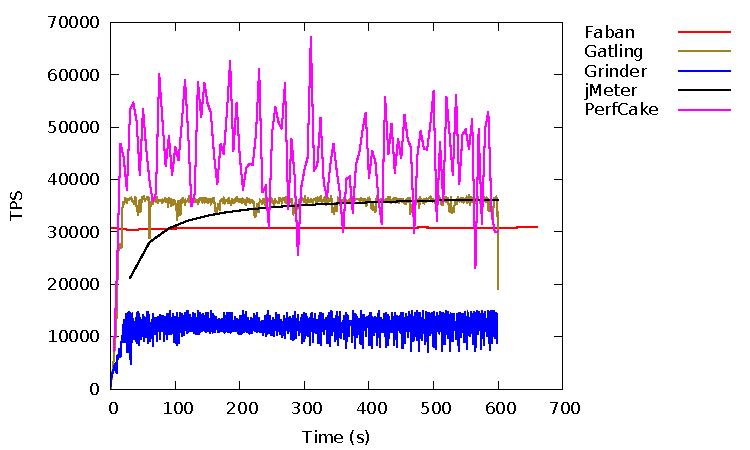
\includegraphics[width=0.75\textwidth]{rest-summary}
    \caption{REST summary}
    \label{fig:rest-summary}
\end{figure}

The SOAP test appeared to perform at approximately the same rate for Faban, Grinder and JMeter, as seen in \autoref{fig:ws-summary}. However, in Gatling, the SOAP test performed almost three times worse than in the other tools, even though it was implemented using the HTTP protocol. The reason for this has not been identified. PerfCake, on the other hand, seemed to significantly outperform the other tools by performing very similarly to HTTP which would be an expected result. 

\begin{figure}[h]
    \centering
    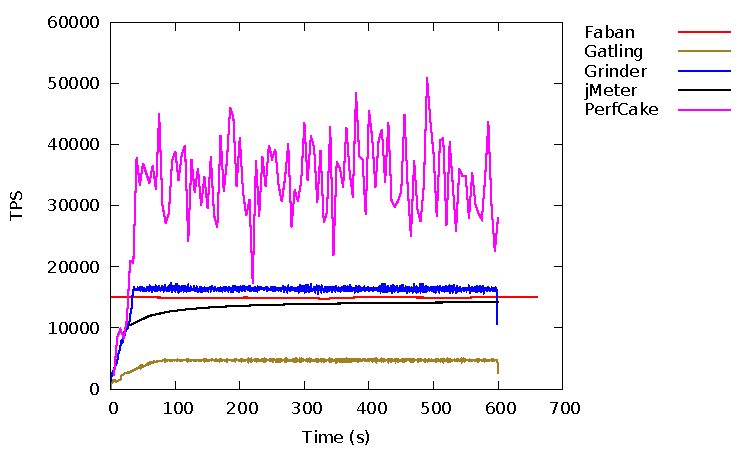
\includegraphics[width=0.8\textwidth]{ws-summary}
    \caption{SOAP summary}
    \label{fig:ws-summary}
\end{figure}


%
%%%%%%%%%%%%%%%%%%%%%
%
%    CHAPTER: TESTING 
%
%%%%%%%%%%%%%%%%%%%%%
%

\chapter{Testing tools applied} \label{chap:testing-tools-applied}
The previous chapter focused on measuring performance characteristics of the tools in a very narrow spectrum of their capabilities in a single discipline -- flooding a server with requests as fast as possible. Choosing the fastest tool might be appropriate mainly for testing the limits of a system or simply to be sure that the testing hardware is being used efficiently. There are however many occasions when other qualities besides rapid load generation are demanded. 

In this chapter we will explore use cases which are closer to real-life use. We chose two of the tools for further testing -- Gatling and PerfCake. These tools share at least one common trait -- they are \textit{modern} in the truest sense. Gatling has seen slightly over 3 years of development and PerfCake not even 2 years which makes them the ``youngest'' among the tested tools. Another common characteristic is the lack of support for using multiple load drivers in one test. That would normally be considered a drawback, however, in this case it turns out to be an advantage, as it provided the opportunity to slightly repurpose the testing environment described in \autoref{sec:environment} and use the \textit{master} machine as a database server instead of a performance test coordinator, which in turn enabled a more realistic deployment of the tested application. 

The following sections will present the application used for testing and its deployment environment, the types of tests implemented and mainly the process of test implementation and the hindrances encountered thereby. 

\section{Application under test}
To provide appropriate proving ground for a modern performance testing tool we set certain requirements for the tested application: it needed to be complex enough as to subject the tested system to some significant and easily measurable load, use some of the technologies supported by the tools and be built on modern web technologies. Based on these requirements an application called \textit{DeltaSpike Expense Tracker}%
\footnote{DeltaSpike Expense Tracker example, sources available at GitHub, \url{https://github.com/rsmeral/deltaspike-examples/tree/master/expense-tracker}. At the time of writing, the application is deployed for demonstrational purposes to OpenShift, \url{http://expensetracker-rsmeral.rhcloud.com}} was chosen.

The application implements basic use cases for corporate expense tracking. It is not publicly used for the purpose stated in its title -- expense tracking -- even though it is a fully functional implementation. Its main purpose is demonstration and testing of features of a project called \textit{DeltaSpike}%
\footnote{\textit{DeltaSpike consists of a number of portable CDI extensions that provide useful features for Java application developers.} \url{http://deltaspike.apache.org/}}.%
From technical viewpoint it is a Java EE 6 application utilizing many of its APIs: CDI 1.0, JPA 2.0, JSF 2.1, Bean Validation 1.0, Servlet 3.0, and several external dependencies: PicketLink IDM, RichFaces, and most of DeltaSpike modules: Core, Security, Data, BeanValidation, JPA, JSF, Servlet, CdiControl. It stores data in two databases, one for domain model data, another for identity model data and has been tested with a MySQL database. 

\section{Testing}
One test scenario was chosen for each of the tools -- a HTTP load test for Gatling with a simulation of a user transaction and a JDBC database stress test for PerfCake with several SQL queries which might occur in the runtime of the application.

\subsection{Gatling HTTP load test}
The Expense Tracker application is covered with functional tests implemented using Arquillian Graphene, an extension of Selenium WebDriver. The aim of functional tests is to simulate the operations of a user as realistically as possible, which is the purpose that WebDriver serves -- it tests an application through a real web browser and automatically performs scripted user operations -- mouse movements, clicks and key presses. Since this is a goal similar on an abstract level to that of workload generation in performance testing where the simulation of user behaviour is one of the key points, this appeared to be worth investigating further.

We initially considered the possibility of integrating the existing functional tests into a Gatling scenario and using them to generate load\footnote{It appears the idea of integrating Arquillian and Gatling is not novel and an Arquillian performance testing extension has been proposed as a project for Google Summer of Code, \url{https://developer.jboss.org/wiki/GSOC14Ideas}}. However, several difficulties obstructed this path. Graphene seems too ``heavy weight'' to use in a case where low overhead is required -- it depends in large part on using JavaScript to inspect and manipulate the web pages, and together with WebDriver adds several layers of abstraction to the process of simulated web navigation. The existing functional tests rely on Graphene in multiple ways -- they use its selectors to match content in responses, its implementation of the \textit{page object} and \textit{page fragment} paradigms and others. A slightly more viable approach would be the significant rewriting of the tests to remove the dependency on Graphene and instead using WebDriver directly, with its simplest driver implementation -- the headless browser HTMLUnit. The abstraction at this level is sufficient to make writing of the scripts fairly trivial, however, at the cost of considerable memory requirements to keep the structures of parsed web pages in memory. Using just HTMLUnit without WebDriver is an option as well though comparable in resource requirements to using WebDriver. The compromise between performance and abstraction seems to be at the level of using an HTTP client.

Gatling's DSL appeared as a way simple and intuitive enough to implement several user transactions. One last option to simplify the scripting was using Gatling's recorder module together with the functional tests -- ``playing'' the test and recording its activity as a script. Due to further complications this approach was not used and instead the captured operations were performed manually. The recorded and ``transcribed'' user session was not immediately usable as a script for several reasons, the prominent being difficulties related to JSF. One problem was the combination of the POST-Redirect-GET\cite{Jouravlev:2004:RedirectAfterPost} pattern and JSF's ViewState, whereby even for simple links, the application would do a POST request with a special form parameter which represents the view state and needs to be propagated between requests. This necessitated a slight modification of every request in the generated script.

Lastly, one significant difference between a functional test and a script for a performance test is the number of virtual users that will be executing that script. In case the application uses some shared resources, which it most likely does, the script can only perform such operations, which do not interfere with other executions of the same script. For example, registering new entities might be simple, but care needs to be taken when deleting them -- the other user could be referring to it.

\subsubsection*{\textbf{Execution}}
The workload consisted of 1 GET request and 16 POST requests representing a simple transaction which spans two user sessions implemented as a single transaction for the sake of simplicity: \textit{Employee logs in, creates an expense report with one expense, submits the report and logs out. Accountant logs in, assigns herself to the report, reimburses the expense, approves the report, marks it as settled and logs out.}

\begin{figure}[h]
    \centering
    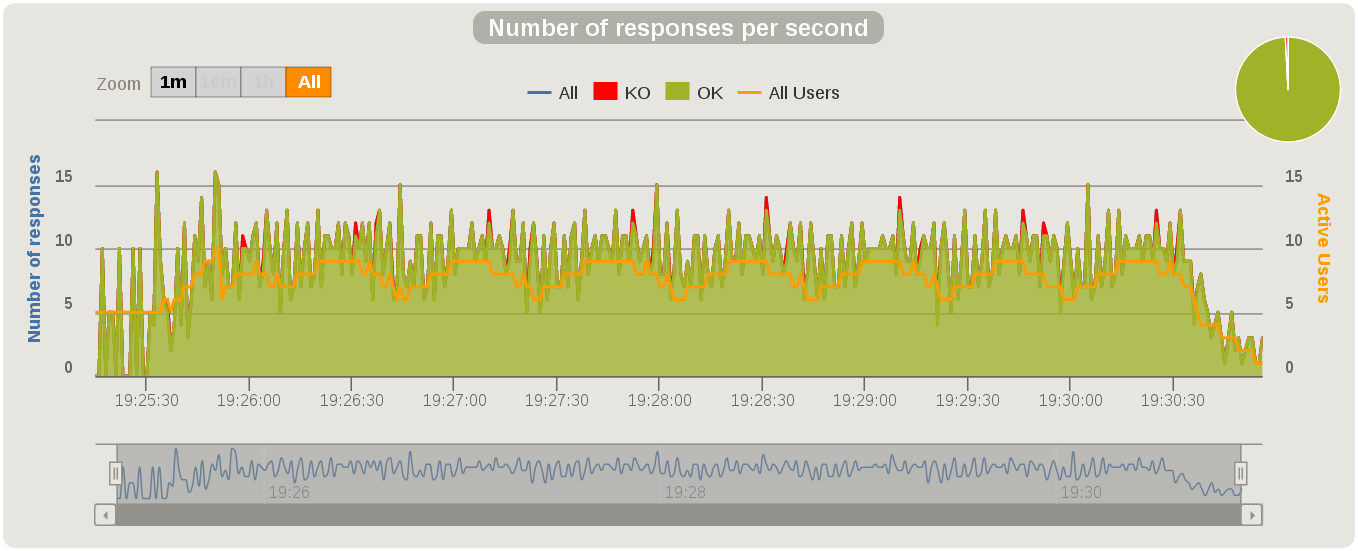
\includegraphics[width=1\textwidth]{gatling-applied-rps-100}
    \caption{Gatling HTTP load test, 100 users over 5 minutes}
    \label{fig:gatling-applied-rps-100}
\end{figure}

The chosen injection profile was an empirically selected combination of profiles: \textit{inject 5 users at once, wait for 20 seconds, then continually inject 100 users over 5 minutes.} The initial burst serves as a warmup period for caches, connection pools and possibly JIT compilation. The resulting average active user count at any second fluctuated between 5 and 10 without any significant bursts or drops and the response count stayed at a similar rate of approximately 10 responses per second, as can be seen in \autoref{fig:gatling-applied-rps-100}. The median response time for the whole run was 521 ms, which is still an acceptable value for an enterprise web application.

\begin{figure}[h]
    \centering
    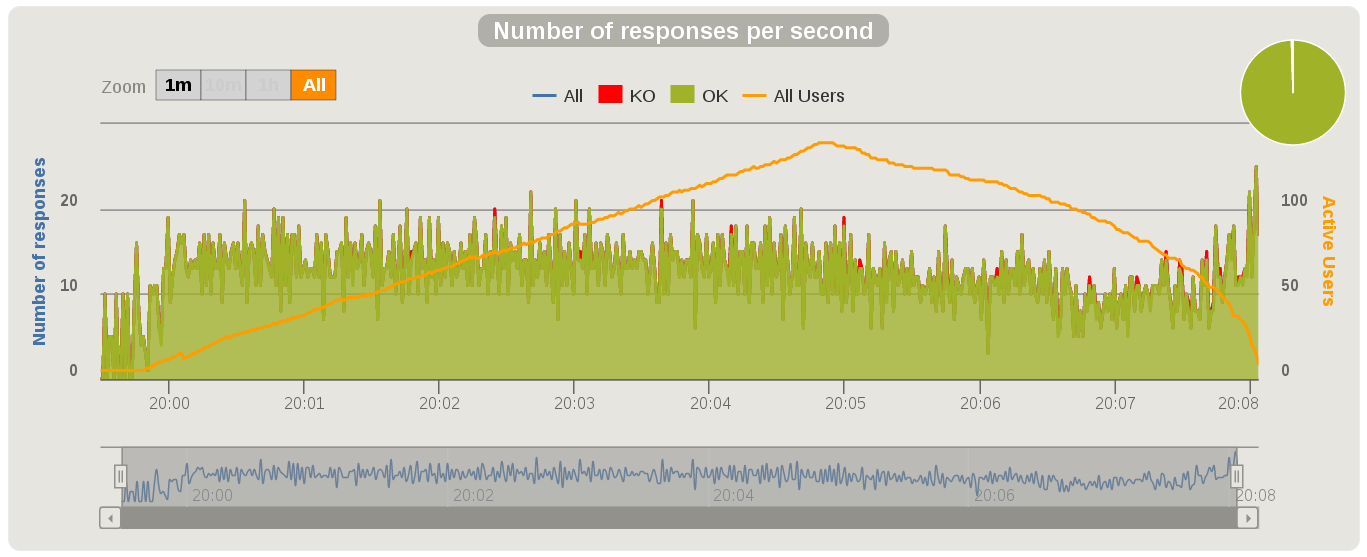
\includegraphics[width=1\textwidth]{gatling-applied-rps-200}
    \caption{Gatling HTTP load test, 200 users over 5 minutes}
    \label{fig:gatling-applied-rps-200}
\end{figure}

For the sake of comparison, we tried increasing the number of injected users to 200, which was apparently beyond the breaking point of the server, as demonstrated in \autoref{fig:gatling-applied-rps-200}. The median response time has seen a 6-fold increase to 3476 ms and the maximum spiked up to 60 seconds for some requests as the server was at peak load of 100 active users at the same time.

All these information were easy to obtain from Gatling's HTML report which contains interactive charts of several metrics and statistics for the whole run, as well as a breakdown by groups and by requests.

\subsection{PerfCake JDBC stress test}
Working with PerfCake's XML scenario format turned out to be fairly straightforward and the configuration of a \texttt{JdbcSender} was simple. The documentation is still slightly lacking and, for example, the conclusion that the message files can only contain one statement each had to be arrived at experimentally. 

The chosen \texttt{RampUpDownGenerator} initially presented several obstacles. In the used PerfCake version 3.3 the generator turned out to have a bug which resulted in a \texttt{NullPointerException} and prevented functionality completely. Thankfully, this has already been fixed in the development branch and therefore a patched 3.3 version of PerfCake was used for testing. Another signal indicating that this generator -- along with many other parts of the code -- is still under active development was the overabundant logging coming from the generator which flooded the console and logs with too many log statements about the current state of the generator\footnote{\url{https://github.com/PerfCake/PerfCake/issues/166}}.

\subsubsection*{\textbf{Execution}}
The workload consisted of 6 different SQL statements executed sequentially and repeatedly by each thread: inserting an employee, selecting all employees, inserting a purpose, selecting all purposes, inserting an expense report, selecting all expense reports. 

From the two supported injection profiles, the ramp-up-down profile was chosen and configured in the following way: \textit{stay at 1 thread for 10 seconds, ramp up to a 100 threads stepping by 2 each second, stay at 100 threads for 200 seconds, ramp down to 20 threads stepping by 4 each second, with a total duration limit of 300 seconds}.

\begin{figure}[h]
    \centering
    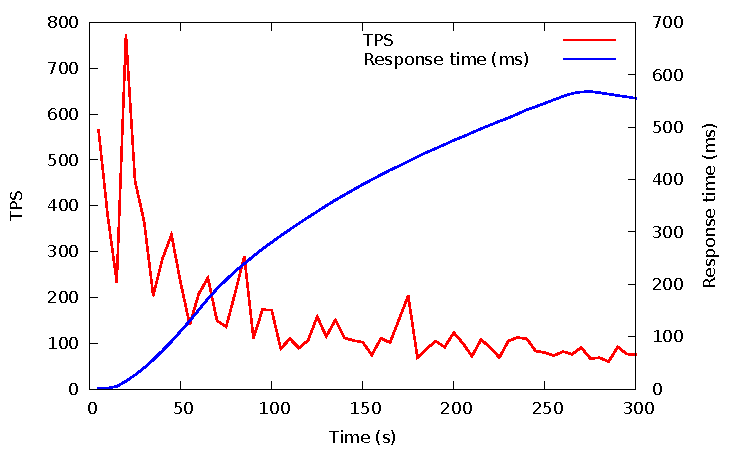
\includegraphics[width=0.8\textwidth]{perfcake-applied-tps-response}
    \caption{PerfCake JDBC stress test, TPS and response time}
    \label{fig:perfcake-applied-tps-response}
\end{figure}

The test has clearly shown a noticeable difference between the performance of an empty database and one that is filled with data. The response time has increased from near-zero to almost 600 ms and the transaction rate has dropped from hundreds to tens. Sadly, PerfCake currently doesn't seem to offer any working mechanism for visual reporting. The plot in \autoref{fig:perfcake-applied-tps-response} was generated manually from the CSV data reported from PerfCake.

\section{Discussion}
The tools Gatling and PerfCake were indeed not the only ones among the tested tools suitable for the tasks described in this chapter. For example, JMeter, Faban or Grinder were just as much -- some maybe even more -- capable of performing the web load test, but Gatling was chosen for the specific reasons noted in the beginning of this chapter. PerfCake was the only tool which despite its other qualities greatly lacks in workload characterization and transaction scripting features and was therefore considered inadequate. However, it still appeared to be a tool worth investigating and was therefore applied in a test for which it seemed to be the most suitable -- stressing a database with as little overhead as possible. 

%
%%%%%%%%%%%%%%%%%%%%%
%
%    CHAPTER: CONCLUSION
%
%%%%%%%%%%%%%%%%%%%%%
%

\chapter{Conclusion} \label{chap:conclusion}
The goal of this thesis was to explore the state of the art in performance testing of web applications and to compare tools designed for that purpose. 

Five tools were the object of investigation: Faban, Gatling, Grinder, JMeter and PerfCake. They were first compared qualitatively and subjectively in several categories: architecture, protocol support, workload definition capabilities, injection profile support, usability, monitoring and reporting capabilities. Significant differences were found among the tools and the total time since inception of the project seems to be somewhat correlated to the breadth of its feature set. The oldest tool JMeter seems to be the most equipped. 

The chosen tools were subjected to analysis of their performance characteristics in four test scenarios: HTTP GET request, REST GET request, JMS request-response and SOAP invocation. The testing was performed in a controlled environment using three powerful server machines and a Jenkins instance for build control. The tests have again shown noticeable differences in performance among the tools and also among protocols of individual tools. On average, the fastest tool appears to be PerfCake.

Two of the tools -- Gatling and PerfCake -- were chosen for further analysis in a test of a real application. Both have proved to be adequate for the job -- Gatling has provided useful visualization which helped identify the maximal load of the application and PerfCake has served well in demonstrating a clear relationship between the number of entries in the database and its response time.


\bibliographystyle{plain}
\bibliography{bib-db}

\appendixchapter{Contents of the attached CD}\label{app:cd}
\begin{itemize}
	\item[\textbf{\texttt{echoapp}}:] The sample application from \autoref{subsec:sample-app}
	\item[\textbf{\texttt{expense-tracker}}:] The application tested in \autoref{chap:testing-tools-applied}
	\item[\textbf{\texttt{jenkins}}:] Configurations of Jenkins jobs and 3 last builds with results
	\item[\textbf{\texttt{results}}:] Aggregated measurement data and gnuplot files
	\item[\textbf{\texttt{scripts}}:] Bash scripts used by Jenkins jobs to manage the tools
	\item[\textbf{\texttt{test-configurations}}:] Test scenario implementations
	\item[\textbf{\texttt{ws-client}}:] The generated Web Service client used in test scenarios
\end{itemize}

\end{document}
